\documentclass[border=2pt]{standalone}
%%
%% Use this file to regenerate tikz diagrams by building the pdf and converting to SVG.
%%
%%     lualatex -halt-on-error -interaction=batchmode STS-Diagram.tex
%%     dvisvgm --pdf --page=1 -n -a -o STS-Diagram.svg STS-Diagram.pdf
%%     cp STS-Diagram.svg ../md/common/src/img/
%%
%% (`--pdf` tells `dvisvgm` to read the PDF, `-n` outlines text so the svg file is
%% self-contained, `-a` preserves transparency)
%%
%% Use the resulting .svg file in a Markdown file as follows:
%%
%%     ![STS-Diagram](img/STS-Diagram.svg)
%%
\usepackage{pgfplots}
\usepackage[tikz]{bclogo}
\usepackage{tikz-cd}
\usetikzlibrary{ arrows.meta
               , backgrounds
               , calc
               , decorations.pathreplacing
               , fit
               , positioning
               , shadows
               , shapes.geometric
               , shapes.misc
               }
\usepackage[dvipsnames]{xcolor}
\usepackage{caption}

\begin{document}
\def\AlonzoColor{Periwinkle}
\def\BabbageColor{Tan}
\def\ConwayColor{yellow!50}
\def\ShelleyColor{lightgray}
\newcommand{\legendbox}[1]{%
  \textcolor{#1}{\rule{\fontcharht\font`X}{\fontcharht\font`X}}%
}
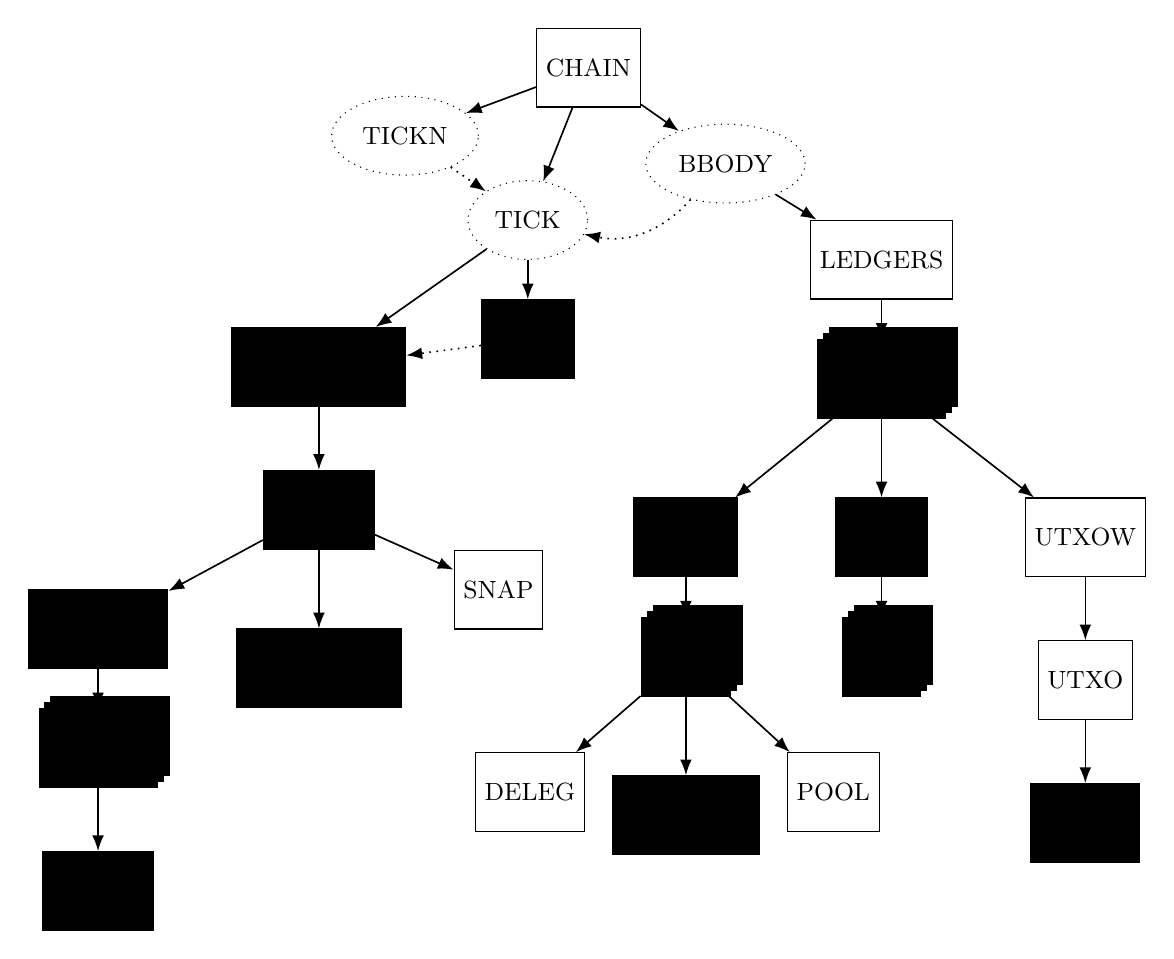
\begin{tikzpicture} [
    conway/.style = {draw, minimum size=1cm, align=right, fill=\ConwayColor},
    shelley/.style = {draw, minimum size=1cm, align=right},
    modified/.style = {draw, minimum size=1cm, align=right, fill=\BabbageColor},
    missing/.style = {draw, ellipse, dotted, minimum size=1cm, align=center},
    dcs/.style = {double copy shadow, shadow xshift=2pt, shadow yshift=-2pt},
    dotted edge/.style={draw, ->, >=Latex, dotted, semithick},
    every edge/.style={draw, ->, >=Latex, semithick}
    ]
  \node[shelley]       (chain)                                            {\small CHAIN};
  \node[missing]       (tickn)   [below left  = 0mm and 1cm  of chain]    {\small TICKN};
  \node[missing]       (bbody)   [below right = 5mm          of chain]    {\small BBODY};
  \node[missing]       (tick)    [below right = 5mm          of tickn]    {\small TICK};
  \node[modified]       (rupd)    [below       = 5mm          of tick]     {\small RUPD};
  \node[modified]      (newepoch)[below left  =              of tick]     {\small NEWEPOCH};
  \node[modified]      (epoch)   [below       = 8mm          of newepoch] {\small EPOCH};
  \node[conway]        (ratifies)[below left  = 5mm and 12mm  of epoch]    {\small RATIFIES};
  \node[modified]       (poolreap)[below       =              of epoch]    {\small POOLREAP};
  \node[shelley]       (snap)    [below right = 0cm and 1cm  of epoch]    {\small SNAP};
  \node[conway, dcs]   (ratify)  [below       = 5mm          of ratifies] {\small RATIFY};
  \node[conway]        (enact)   [below       = 8mm          of ratify]   {\small ENACT};
  \node[shelley]       (ledgers) [below right = 5mm          of bbody]    {\small LEDGERS};
  \node[modified, dcs] (ledger)  [below       = 5mm          of ledgers]  {\small LEDGER};
  \node[conway]        (certs)   [below left  =              of ledger]   {\small CERTS};
  \node[conway]        (govs)    [below       =              of ledger]   {\small GOVS};
  \node[shelley]       (utxow)   [below right =              of ledger]   {\small UTXOW};
  \node[conway, dcs]   (cert)    [below       = 5mm          of certs]    {\small CERT};
  \node[shelley]       (utxo)    [below       = 8mm          of utxow]    {\small UTXO};
  \node[conway, dcs]   (gov)     [below       = 5mm          of govs]     {\small GOV};
  \node[shelley]       (deleg)   [below left  = 1cm          of cert]     {\small DELEG};
  \node[conway]        (govcert) [below       =              of cert]     {\small GOVCERT};
  \node[shelley]       (pool)    [below right = 1cm          of cert]     {\small POOL};
  \node[modified]      (utxos)   [below       = 8mm          of utxo]     {\small UTXOS};

\draw
  (chain)    edge                         (tick)
  (chain)    edge                         (tickn)
  (chain)    edge                         (bbody)
  (tickn)    edge[dotted edge]            (tick)
  (tick)     edge                         (newepoch)
  (tick)     edge                         (rupd)
  (bbody)    edge                         (ledgers)
  (bbody)    edge[dotted edge, bend left] (tick)
  (rupd)     edge[dotted edge]            (newepoch)
  (newepoch) edge                         (epoch)
  (epoch)    edge                         (ratifies)
  (epoch)    edge                         (snap)
  (epoch)    edge                         (poolreap)
  (ratifies) edge                         (ratify)
  (ratify)   edge                         (enact)
  (ledgers)  edge                         (ledger)
  (ledger)   edge                         (certs)
  (ledger)   edge                         (govs)
  (govs)     edge                         (gov)
  (ledger)   edge                         (utxow)
  (certs)    edge                         (cert)
  (cert)     edge                         (deleg)
  (cert)     edge                         (pool)
  (cert)     edge                         (govcert)
  (utxow)    edge                         (utxo)
  (utxo)     edge                         (utxos);
  \end{tikzpicture}

\end{document}
